\section{Модель системы передачи с криптозащитой}
\selectlanguage{russian}

Простая модель системы передачи с криптозащитой представлена на рис.~\ref{pic:Encrypt}, где введены следующие обозначения:
\begin{itemize}
    \item $A$ -- источник информации;
    \item $B$ -- получатель информации, легальный пользователь;
    \item $X$ -- сообщение до шифрования или \emph{открытый текст}\index{открытый текст} (\langen{plaintext}); $\set{M}$ -- множество всех возможных открытых текстов (от слова Message), $X \in \set{M}$;
    \item $K_1$ -- ключ шифрования\index{ключ!шифрования} (\langen{encryption key}); $\set{K}_E$ -- множество всех возможных ключей шифрования, $K_1 \in \set{K}_E$;
    \item $Y$ -- зашифрованное сообщение (\emph{шифротекст}\index{шифротекст}, \langen{ciphertext, cyphertext} или \emph{шифрограмма}\index{шифрограмма}\footnote{Строго говоря, \emph{шифрограмма} -- это \emph{шифротекст} после его \emph{кодирования} для целей передачи по каналу связи}); $\set{C}$ -- множество всех возможных шифротекстов, $Y \in \set{C}$;
    \item $K_2$ -- ключ расшифрования\index{ключ!расшифрования} (\langen{decryption key}); $\set{K}_D$  -- множество возможных ключей расшифрования, зависящее от множества $\set{K}_E$, $K_2 \in \set{K}_D$.
\end{itemize}

\begin{figure}[!thb]
	\centering
	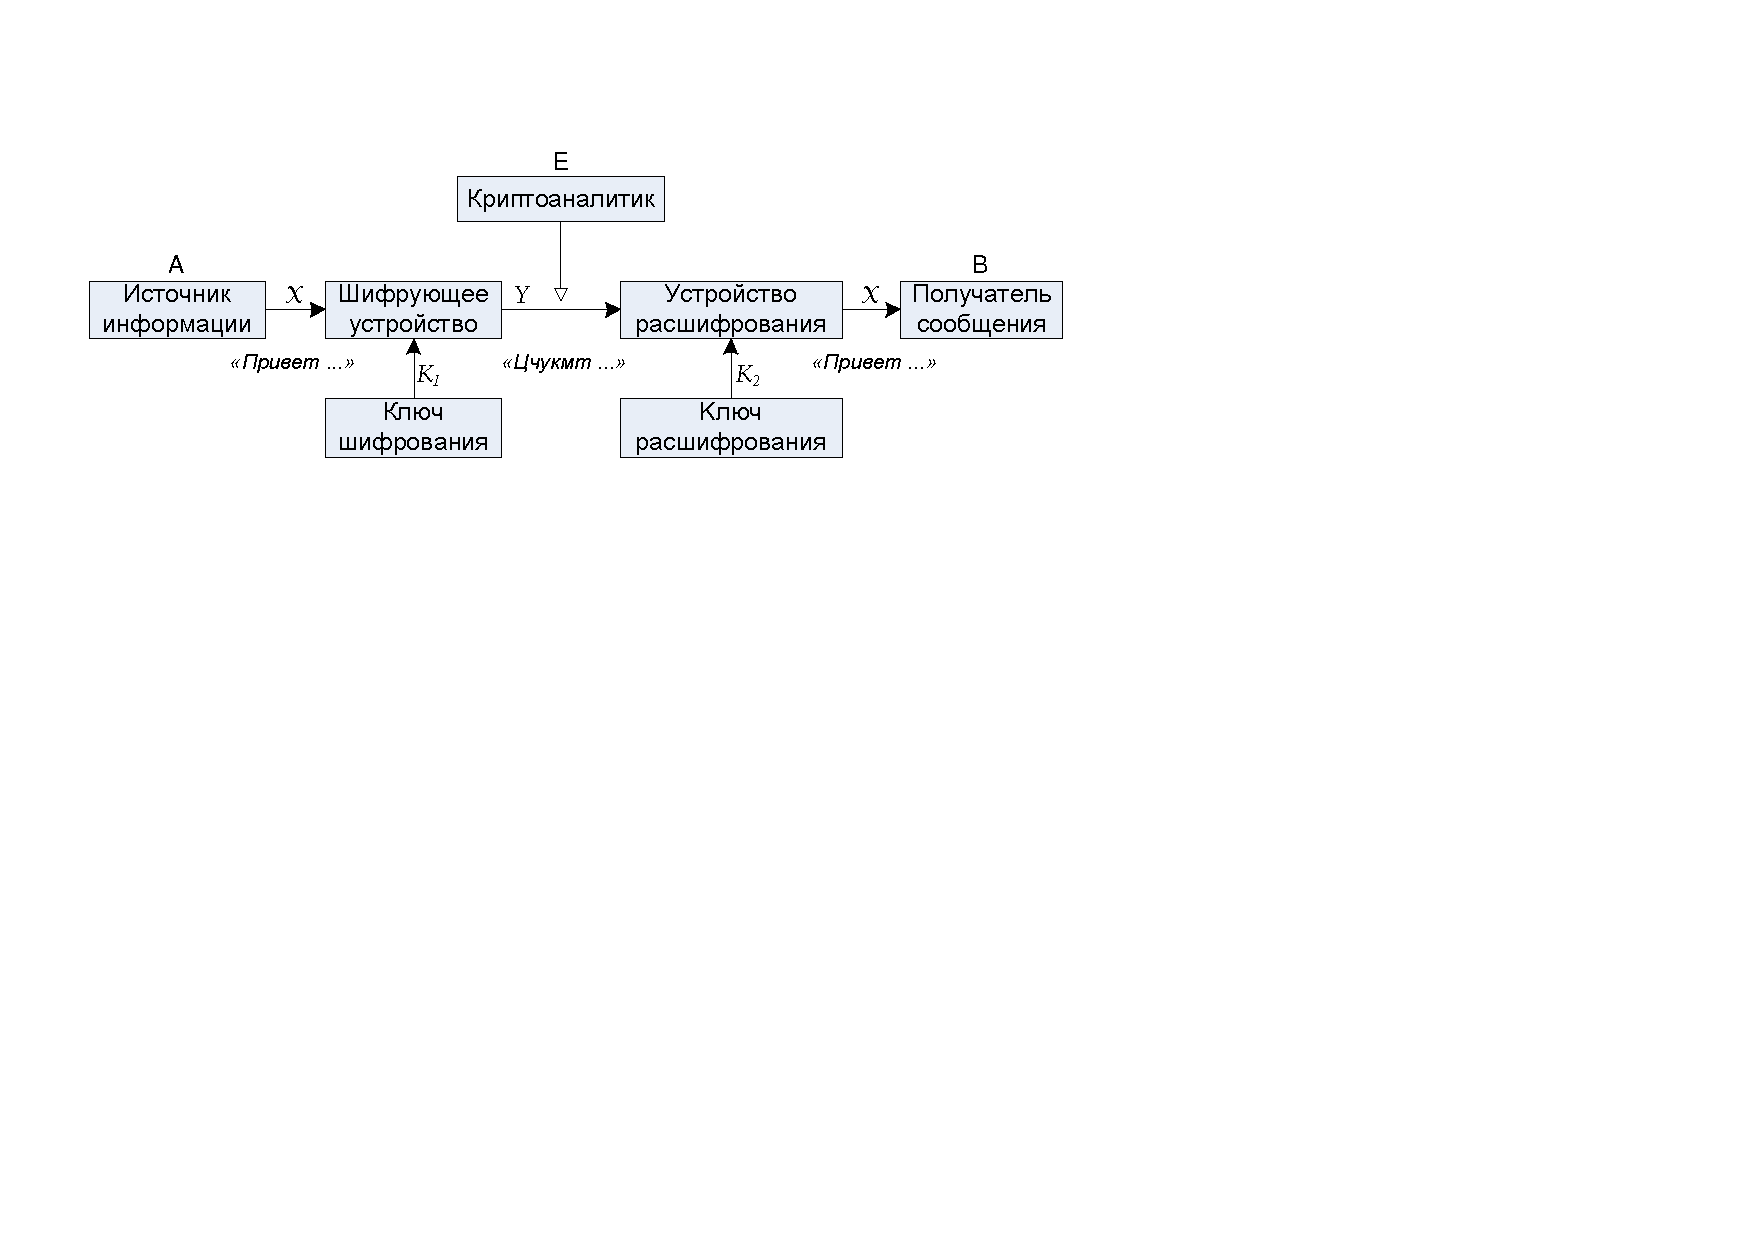
\includegraphics[width=1.0\textwidth]{pic/scheme-of-cipher}
	\caption{Передача информации с криптозащитой\label{pic:Encrypt}}
\end{figure}

\emph{Шифр}\index{шифр} -- это множество обратимых функций отображения $E_{K_1}$\index{функция!шифрования} множества открытых текстов $\set{M}$ на множество шифротекстов $\set{C}$, зависящих от выбранного ключа шифрования $K_1$ из множества $\set{K}_E$:
%обратимое отображение пары из элемента множества открытых текстов $\set{M}$ и элемента множества ключей шифрования $\set{K}_E$ в множество шифротекстов $\set{C}$:
\begin{equation}
    \label{eq:Encryption}
    Y = E_{K_1}(X), ~ X \in \set{M}, ~ K_1 \in \set{K}_E, ~ Y \in \set{C}.
\end{equation}
Можно сказать, что шифрование -- это обратимая функция двух аргументов: сообщения и ключа. Для каждого $K_1$ эта функция должна быть обратимой. Обратимость -- основное условие шифрования, по которому каждому зашифрованному сообщению $Y$ и ключу $K$ соответствует одно исходное сообщение $X$. Легальный пользователь $B$ (на приемной стороне системы связи)  получает сообщение $Y$ и осуществляет процедуру \emph{расшифрования}\index{расшифрование}.
Следует отличать шифрование от кодирования, так как кодирование -- это процесс сопоставления конкретным сообщениям строго определенной комбинации символов или сигналов, с целью повышения помехоустойчивости передаваемого сигнала.
Расшифрование --  это отображение множества шифротекстов $\set{C}$ в множество открытых текстов $\set{M}$ функцией $D_{K_2}$\index{функция!расшифрования}, зависящей от ключа расшифрования $K_2$ из множества $\set{K}_D$, являющейся обратной к функции $E_{K_1}$.
\begin{equation}
    \label{eq:Decryption}
    D_{K_2}(Y) = X, ~ Y \in \set{C}, ~ K_2 \in \set{K}_D, ~ X \in \set{M}.
\end{equation}

%Система передачи информации с криптозащитой называется \emph{криптосистемой}\index{криптосистема}.(?????)

%В общем случае функция шифрования сюръективна и псевдослучайна, отображая один открытый текст в разные шифротексты. Если функция шифрования биективна, на практике ее инкапсулируют в другую функцию с целью добиться псевдослучайности шифрования одинаковых открытых текстов в разные шифротексты.

%Методы защиты информации зависят от возможных сценариев передачи. Рассмотрим несколько основных вариантов.
Рассмотрим возможные сценарии вмешательства криптоаналитика и организации защиты информации от его действий.
Пусть  $A$ --  источник и $B$ -- получатель сообщений.

\begin{description}
    \item[Сценарий 1.] Пусть $E$ -- \emph{пассивный} криптоаналитик\index{криптоаналитик!пассивный}, который может подслушивать передачу, но не может вмешиваться в процесс передачи. Из пассивности криптоаналитика следует, что $Y = \widetilde{Y}$, и \emph{целостность} информации обеспечена.

Цель защиты --- \emph{обеспечение конфиденциальности}.

Средства защиты -- шифрование с помощью \emph{симметричных} или \emph{асимметричных } криптосистем.

Дополнительные задачи -- при большом числе пользователей должна быть решена задача \emph{генерации и доставки секретных ключей} всем пользователям.

    \item[Сценарий 2.] Пусть $E$ -- \emph{активный} криптоаналитик\index{криптоаналитик!активный}, который может изменять, удалять и вставлять сообщения или их части.

    Цель защиты -- \emph{обеспечение конфиденциальности} и  \emph{обеспечение целостности}.

Средства защиты --  шифрование и добавление \emph{имитовставки}\index{имитовставка} (message authentication code -- $\MAC$), позволяющего обнаружить нарушение целостности.

    \item[Сценарий 3.] Пусть $E$ -- активный криптоаналитик, который может изменять, удалять и вставлять сообщения или их части, дополнительно к этому легальные пользователи $A$ и $B$ не доверяют друг другу.

Цель защиты -- \emph{аутентификация} пользователей и документов.

Средства -- \emph{электронная подпись} и протокол идентификации (аутентификации) пользователей.
\end{description}

%%Возможно вмешательство нелегального пользователя $E$, называемого \emph{криптоаналитиком}.
%%
%%
%%Если $X = \widetilde{X}$, то вмешательство криптоаналитика  $E$ не изменило передаваемое сообщение, и \emph{целостность} информации обеспечена. Если криптоаналитик не получил информацию, содержащуюся в сообщении, то обеспечена \emph{конфиденциальность}.
%%
%%Если в этой системе возможна двусторонняя передача, то есть от $A$ к $B$ и от $B$ к $A$, то говорят о взаимном обмене информацией между легальными пользователями.
%
%Секретность информации в современных шифрах обеспечивается секретным ключом, в то время как сам алгоритм криптосистемы является общеизвестным. Исторический опыт, например, система шифрования A5/1 в GSM, показывает, что секретность алгоритма шифрования \emph{ослабляет} криптостойкость шифра, а не увеличивает, из-за того, что система становится малоизученной.
